\newpage
\section{Summe der 7-Tage-Inzidenzen der Landkreise und Regierungsbezirke}
Als letzte in \autoref{sec:Vorgehensweise:Datendarstellung:Allgemeine Daten der Gebiete} angesprochene Kennzahl folgt in diesem Abschnitt die Darstellung der durchschnittlichen 7-Tage-Inzidenz der Landkreise und Regierungsbezirke.
In \autoref{fig:distribution_incidences_counties} sind die Mittel der 7-Tage-Inzidenz der einzelnen Landkreise dargestellt. Auffällig ist hierbei die starke Ausprägung in Sachsen und Thüringen mit einigen Landkreisen mit durchschnittlichen 7-Tages-Inzidenzen über 100 neu gemeldeten Fällen pro 100~000 Einwohnern.

\begin{figure}[H]
    \centering
    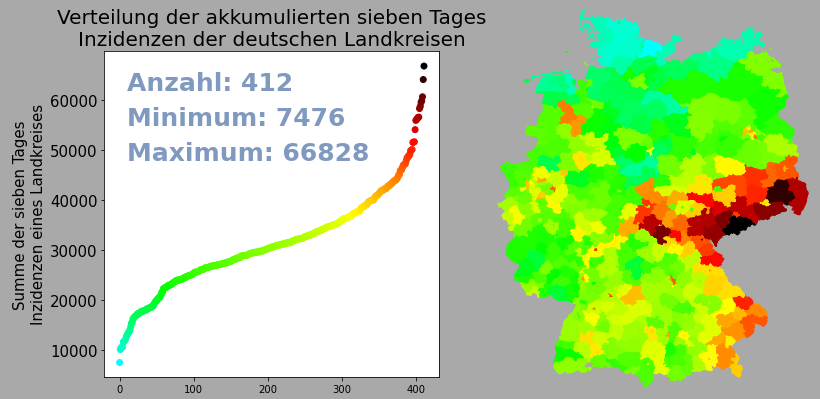
\includegraphics[width = \textwidth]{figures/Ergebnisse/accumulation_incidences_counties.png}
    \caption{Die Verteilung der Mittel der 7-Tage-Inzidenz $\overline{i}$ unter den Landkreisen. Berechnet nach \autoref{eq:Mittelwert} und \autoref{eq:7-Tages_Inzidenz}.
    Auf der linken Seite befindet sich die Verteilung, welche zudem die Farbgebung vorgibt. Auf der rechten Seite befindet sich die räumliche Anordnung. Die Farbgebung entspricht \autoref{sec:Grundlagen:Farbgebung}.}
    \label{fig:distribution_incidences_counties}
\end{figure}
\newpage
In \autoref{fig:distribution_incidences_districts} sind die Mittel der 7-Tage-Inzidenz der einzelnen Regierungsbezirke dargestellt.
Auch hier sind zwei der drei Regierungsbezirke Sachsens Spitzenreiter mit durchschnittlichen 7-Tage-Inzidenz von über 100 neu gemeldeten Fällen in den letzten 7 Tagen pro 100~000 Einwohnern.

\begin{figure}[H]
    \centering
    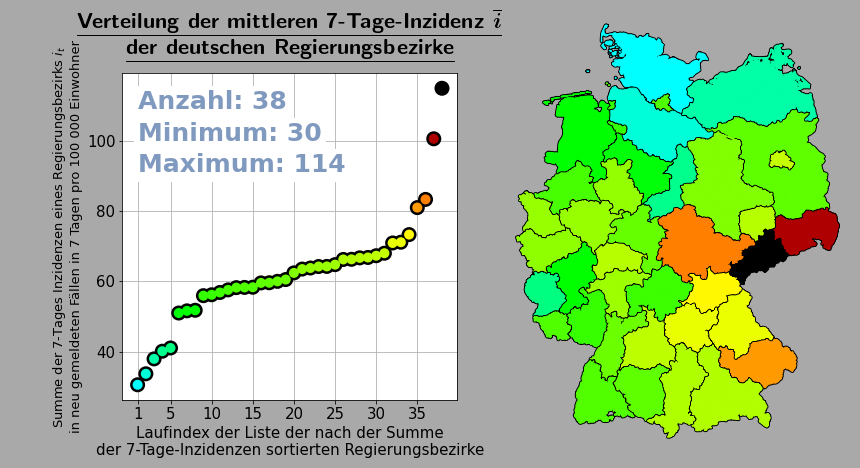
\includegraphics[width = \textwidth]{figures/Ergebnisse/accumulation_incidences_districts.png}
    \caption{Die Verteilung der Mittel der 7-Tage-Inzidenz $\overline{i}$ unter den Regierungsbezirken. Berechnet nach \autoref{eq:Mittelwert} und \autoref{eq:7-Tages_Inzidenz}.
    Auf der linken Seite befindet sich die Verteilung, welche zudem die Farbgebung vorgibt. Auf der rechten Seite befindet sich die räumliche Anordnung. Die Farbgebung entspricht \autoref{sec:Grundlagen:Farbgebung}.}
    \label{fig:distribution_incidences_districts}
\end{figure}